\documentclass[conference]{IEEEtran}
\IEEEoverridecommandlockouts

% ============================================================
% Packages
% ============================================================
\usepackage{cite}
\usepackage{amsmath,amssymb,amsfonts}
\usepackage{algorithm}
\usepackage{algorithmic}
\usepackage{graphicx}
\usepackage{textcomp}
\usepackage{xcolor}
\usepackage{booktabs}
\usepackage{multirow}
\usepackage{siunitx}
\usepackage{hyperref}
\usepackage{pifont}
\usepackage[caption=false,font=footnotesize]{subfig}

% 支持中文排版 (推荐在 Overleaf 中使用 XeLaTeX 编译)
\usepackage[UTF8]{ctex}

% Checkmark and crossmark
\newcommand{\cmark}{\ding{51}}
\newcommand{\xmark}{\ding{55}}

% ============================================================
% Title
% ============================================================
\title{PA-LOI: 面向遮挡横穿主动避撞的速度感知风险场}

% --- Anonymized Author Block for Double-Blind Review ---
\author{\IEEEauthorblockN{Primary Author}
\IEEEauthorblockA{\textit{Author affiliation is anonymized} \\
\textit{for double-blind review.}\\
City, Country \\
email anonymized}
}
% --- End Anonymized Block ---

\begin{document}
\maketitle

% ============================================================
% Abstract
% ============================================================
\begin{abstract}
视线受阻横穿场景 (Occluded Pedestrian Crossing)——即行人突然从视野遮挡物后方显现——对自动驾驶构成了严峻的安全挑战。由于视距传感器只能在行人完全出现后才能检测到目标，导致在典型城市车速下物理制动距离严重不足，仅凭反应式自动紧急制动（AEB）往往无法及时刹停。我们提出了 \textbf{PA-LOI}（基于潜在遮挡推断的主动预判），一种轻量化、模块化的风险感知规划层，它基于物理可达性模型，在检测到任何行人\emph{之前}，就能主动降低自车穿越高危遮挡区域时的速度。与容易引发轨迹振荡和局部死锁的传统空间避障势场不同，PA-LOI 引入了“速度感知合页损失（Hinge-Loss）代价函数”，仅对超出动态安全阈值的超额速度施加惩罚，一旦车速降至安全范围内即可实现零残余梯度与平滑减速。我们在基于 Argoverse 2 数据集构建的两个 Euro NCAP CPNA 代表性场景中验证了 PA-LOI。在十字路口场景中，PA-LOI+AEB 在行人净距仅 \SI{2.25}{\meter} 时实现零碰撞，安全裕度较单独 AEB 提升了 \textbf{31\%}。在单独 AEB 完全失效的高速直道场景中，PA-LOI 仍将最恶劣工况下的碰撞动能降低了约 \textbf{91\%}。该模块每帧规划仅新增 \SI{0.55}{\milli\second} 耗时，满足闭环部署的实时性需求。
\end{abstract}

\begin{IEEEkeywords}
Automatic Emergency Braking, Autonomous Driving, Euro NCAP CPNA, Occluded Pedestrian Crossing, Occlusion-Aware Planning, Risk Field
\end{IEEEkeywords}

% ============================================================
% I. Introduction
% ============================================================
\section{引言 (Introduction)}

弱势道路使用者的安全防护一直是城市智能交通系统研究的关键痛点。其中，由视线受阻引发的弱势群体横穿场景 (Occluded Pedestrian Crossing) 尤为值得关注。这类场景在汽车安全标准中通常被定义为 Euro NCAP 的 CPNA（Car-to-Pedestrian Nearside Adult，车对近端成人）标准测试场景~\cite{euroncap2023}：即行人突然从遮挡物（如路边连续停放的车辆或大型设施）前方的盲区横穿入当前主车道。由于遮挡物的存在，在目标完全暴露在车辆感知视场以内之前，留给系统执行物理规避和制动的时间窗极其有限。

当前主流的自动紧急制动 (AEB) 系统在减少直视追尾和常规视野下的行人冲突方面已展现出显著成效~\cite{cicchino2022effects}。此外，向信息-物理-社会系统（CPSS）和平行驾驶架构的范式转变，极大地推动了智能汽车从被动感知向主动预测和避撞的演进~\cite{wang2024parallel, wang2021review}。然而，当面对极近距离内突然出现的视野盲区切入者时，AEB 系统的底层逻辑存在严重的局限性。\textbf{AEB 的固有局限性不在于感知延迟，而在于物理上不可能在极近距离内从高速状态下完全刹停。} 因为在当前主流的基于视距的感知体系（摄像头与激光雷达）下，传感器只有在行人完全脱离遮挡物的遮蔽后才能确认其存在。在 CPNA 场景中，此时行人与车辆的可用净距通常仅为 2$\sim$4 米。而以典型城市巡航速度 \SI{8.0}{\meter\per\second} 计，即便使用保守的减速度假设（$a_{\text{max}} = \SI{-4.0}{\meter\per\second\squared}$），最小运动学制动距离也高达 \SI{8.0}{\meter}——远超可用净距的两倍。这一运动学矛盾无法单纯通过提升感知算法的灵敏度来弥补；唯有在进入遮挡区域\emph{之前}主动进行速度管理，才能从根本上扩大 AEB 的有效工作包络。

由此，我们提出了 \textbf{PA-LOI} 框架。本研究的技术贡献如下：
\begin{enumerate}
    \item 提出了一种基于到达时间（TTA）的物理可达性评估与防守车速 ($v_{\text{safe}}$) 动态界定机制。系统通过运动学模型反推行人的威胁时间窗，并以此建立交汇前的安全车速包络界限。该机制精确剥离了对非实质性碰撞威胁的过度干预，在满足底层制动需求的前提下最大限度缓解了前置规划层易发的“幽灵刹车”问题，有效平衡了安全性与通行效率；
    \item 提出了一种以速度解耦的合页损失（Hinge-Loss）动态风险场代价函数，打破了传统空间排斥势场在受限车道（如单车道或实线约束）内易引发轨迹震荡及陷入局部优化死锁的局限性；
    \item 成功在基于最优控制的闭环高频规划器中完成了该主被动联合模块的轻量化部署验证，实验测得 PA-LOI 单帧平均额外耗时仅约 \SI{0.55}{\milli\second}。新方案得益于惩罚分区的闭式解析与平滑可导特性，与求解器的偏导推演高度契合，为未知盲区环境下的碰撞风控提供了高效且极具泛化性的架构参考。
\end{enumerate}

该框架可作为独立的主动风控层，与目前基于最优控制 (Optimal Control) 的多类轨迹寻优算法实现平滑集成。

% ============================================================
% II. Related Work
% ============================================================
\section{相关工作 (Related Work)}

\subsection{自动紧急制动 (AEB) 与安全防线测试}
提升在不确定环境下的弱势群体安全性是高级辅助驾驶系统发展的重心。Euro NCAP 近年来持续深化了以 CPNA 为代表的视线受阻场景测试方案并提出了严苛标准~\cite{euroncap2023}。实证表明，由于侧翼遮挡物导致感知预留期缩短，部分配置 AEB 的车辆在此类极端场景中依然存在较高的碰撞概率~\cite{cicchino2022effects}。Schratter 等人~\cite{schratter2019occlusion} 专门针对遮挡场景提出了一种基于 POMDP 的行人防碰撞系统，强调了在此类环境中超越反应式制动、进行主动决策的根本需求。这些发现共同为在规划前端引入速度主动干预管控思路奠定了理论支持。

\subsection{视野盲点与遮挡感知运动规划}
在运动规划中处理不确定性遮挡问题已吸引了多种方法论视角的广泛关注。Orzechowski 等人~\cite{orzechowski2018tackling} 率先提出了基于集合的安全验证方法以处理有限的传感器范围和遮挡区域，而 Koschi 和 Althoff~\cite{koschi2021setbased} 将其扩展为一个综合框架，使用结合了遮挡与交通规则的正式可达性分析来预测可见和隐藏的交通参与者。Nager 等人~\cite{nager2019shadows} 提出了意图感知的动态阴影区域，实现了计算高效的遮挡区域安全推理。更近地，M\"{o}ller 等人开发了 FRENETIX-Occlusion 框架~\cite{blindspot2024} 及其用于城市遮挡跟踪的后续版本~\cite{occtrack2025}，将虚拟目标建模直接嵌入了轨迹评估管道中。

从决策理论的角度来看，责任敏感安全模型 (RSS)~\cite{shalev2017rss} 在最坏情况假设下提供了保守的安全驾驶边界，但过度应用会使驾驶过于谨慎且缺乏实用性。基于部分可观测马尔可夫决策过程 (POMDP) 的规划器~\cite{zhang2021pomdp} 提供了处理部分可观测性的原则性方法，但会产生巨大的计算开销。近期的概率学方法，例如 Chen 等人~\cite{chen2023quantified} 在 ITSC 2023 展出的虚拟障碍物随机模型预测控制 (Stochastic MPC) 框架，量化了遮挡风险并规划了平衡安全性与效率的轨迹。更宽泛地，基于场景化模型预测控制在高速公路和城市驾驶环境下的不确定性安全决策中也被证明是有效的~\cite{cesari2017mpc}。此外，理解行人语义，特别是过街意图，对于优化安全边界至关重要。为了根据骨骼姿态和时空线索准确推理横穿意图，尹守国等~\cite{yin2026pedestrian} 与王飞跃等~\cite{wang2024parallel} 分别提出了基于多特征融合的推理框架及平行驾驶研究，强调了高保真人体状态推断在自动驾驶安全中的重要性。

需要指出的是，PA-LOI 与上述方法并不处于同一抽象层级。\textbf{尽管这些方法解决了部分可观测条件下的通用遮挡问题，但 PA-LOI 针对的是一个特定的、具有高影响力的子问题，并提供了一种轻量级、工程友好的解决方案}——在已知遮挡结构下且单帧运算预算 $< \SI{1}{\milli\second}$ 内，管理单一横穿威胁的安全车速。此外，综合性的概率求解方案或虚拟目标跟踪框架通常需要显著更高的计算预算，因此在我们亚毫秒级的限制下进行直接的基线对比是不公平的。

\subsection{风险势场与动能惩罚解耦}
传统的人工势场法~\cite{khatib1986potential} 在轨迹优化中常构建虚拟斥力场来规避静态和动态障碍。然而，“距离越近排斥力越大”的传统空间排斥势能一旦置于狭窄且包含对向车流甚至实线隔离的双向盲区环境内，会因横向强避让力驱使车辆产生反复横摆的振荡轨迹，乃至使迭代规划器困于局部极小值死锁。PA-LOI 则将横向空间距离降格为纯粹的标量权重乘子（通过 Sigmoid 衰减），而彻底消除了位置维度上的梯度输出，转而构建以超额速度（即自车速度超出安全阈值 $v_{\text{safe}}$ 的部分）为唯一惩罚对象的专供损失函数。\textbf{Hinge-Loss 公式确保了当 $v_{\text{ego}} \leq v_{\text{safe}}$ 时梯度精确为零，从而将速度控制与空间约束解耦，并避免了空间势场固有的局部极小值问题。}这一特性使得有效压制超速与保留平稳轨迹两个目标得以兼容并行。

% ============================================================
% III. System Architecture
% ============================================================
\section{系统架构 (System Architecture)}

在本文中，PA-LOI 被配置为主被动防御架构中的轻量化中间件。我们将其实例化部署于最先进的自动驾驶规划框架 MIND~\cite{mind2025}。原版 MIND 具备强大的多模态意图预测与交互决策能力，但并未内置针对长尾未知遮挡区域的风险推断机制。PA-LOI 被平行挂载于 MIND 核心的迭代线性二次调节器 (iLQR) 算法旁，其输出的特化风险代价直接进入主预测模块，并与下方的底层触发元件（如 常规 AEB）协同，从而填补了原系统在视野盲点防范上的空白。

\subsection{基于物理降频衰减的威胁评估}
为避免因识别到任意停止车辆即执行强制制动的过度保守行为，PA-LOI 首先构建了一套基于物理学基础判据的权重衰减与安全车速 ($v_{\text{safe}}$) 解析模型。

当感知系统捕捉到路侧具备视线截断效应的静态物体时，PA-LOI 随即锚定一个朝向自车行驶车道的假想源提取点（Target Point），用以标定由于视线受阻可能突然出现的危险发生源位置。随后，分别计算自车顺车道前进直至抵达目标临界截面的到达预期时间（$TTA_{\text{ego}}$）。
根据机制设定，该特定风险的紧迫权重 $w_{\text{base}}$ 表现为针对 $TTA_{\text{ego}}$ 的衰减函数——若估计自车抵达时间过远（即超过远场边界 $TTA_{\text{ego}} > 6.5\text{s}$），系统将其裁定为非即时接触威胁，强制设定 $w_{\text{base}} = 0$。需要强调的是，该 $\SI{6.5}{\second}$ 阈值并非经验预设，而是基于运动学物理界限与 ADAS 工程标准的严密推导。在测试设定的 \SI{8.0}{\meter\per\second} 行驶车速（约 30 km/h，为国际通用的城市视线遮挡区、居住区安全限速标准）下，将其平缓降至约 \SI{2.5}{\meter\per\second} 的防御脱困速度存在 \SI{5.5}{\meter\per\second} 的速度差。为确保乘客舒适度并避免乘员前倾，要求减速度维持在趋近 \SI{-1.0}{\meter\per\second\squared} 的区间——该数值远在 ISO 15622 适应性巡航 \SI{-3.5}{\meter\per\second\squared} 舒适极限以内。这一纯运动学减速过程即需消耗 \SI{5.5}{\second}。

更为关键的是，我们还必须额外吸纳符合 ADAS 工程标准的不可压缩 \SI{1.0}{\second} 系统综合延迟冗余，其构成为：感知与多目标跟踪 (MOT) 收敛（约 $\sim\!\SI{0.3}{\second}$）；控制通讯与规划结算（约 $\sim\!\SI{0.2}{\second}$）；以及机械制动器建压响应（约 $\sim\!\SI{0.5}{\second}$）。

将 \SI{5.5}{\second} 的运动学耗时与 \SI{1.0}{\second} 的系统迟滞相加，精确地从物理层面构成了这 \SI{6.5}{\second} 的前置防御视界。而随着车辆估计到达时间 $TTA_{\text{ego}}$ 跌破该阈值并持续减小，$w_{\text{base}}$ 则开始逐步形成线性上升的响应梯度。
在此之前，系统还设置了空间层面的前置筛选：若目标点已位于自车身后（纵向投影为负），或其横向距离超出当前车道动态走廊的外边界，则该候选风险源将被直接剔除，不参与后续的权重分配与势场构建。该筛选机制确保仅有处于自车前方且横向上具备物理交汇可能性的遮挡点才会进入代价函数。

除此之外，为真正实现对通行效率和平顺性的双向保全，PA-LOI 第二道机制着眼于动态防守底线 $v_{\text{safe}}$ 的解算：
通过获取当前障碍物掩体与自车轨迹中心线的待冲刺横向偏离物理距离 $d_{\text{ped}}$ ，并采用快走或慢跑的标准评估假设 $v_{\text{ped}} = \SI{2.0}{\meter\per\second}$，反推出行人完全横切暴露所需的跨界反应时间 $t_{\text{react}} = d_{\text{ped}} / v_{\text{ped}}$。为确保进入盲区的自车有充分余裕在场景设定的可用制动减速度 $a_{\text{max}}$ 的作用下于制动距离内刹停，自车被安全允许跨越该切面的最高物理速度界限为 $v_{\text{safe\_physics}} = |a_{\text{max}}| \cdot t_{\text{react}}$。

这一公式设计具备天然的自适应调节特性：若当前车道本身十分宽阔（即由于 $d_{\text{ped}}$ 大而带来的反应冗余较长），则其演算获取的 $v_{\text{safe}}$ 指标将会自动放大至极宽容区间。结合后续引入的势场设计，当其阈值覆盖住自车当前合理的正常巡航速度时，就不会产生额外的降速约束拉扯，从而在机制根源上杜绝了对非敏感目标“幽灵刹车”动作的生成。
此外，为防止在极端近距工况（$d_{\text{ped}}$ 极小）下物理公式输出过低的 $v_{\text{safe}}$ 而引发突兀的急制动，系统额外设置了双层防护机制。首先是舒适性阻尼边界 $v_{\text{safe}} \geq 0.6 \cdot v_{\text{ego}}$，该约束将每次规划周期内呈现给 iLQR 优化器的速度惩罚代价井深限制在当前车速的 $40\%$ 以内。这一设计从源头上阻止了优化器因临时激活的风险场产生大幅度的突变减速指令：通过约束 $v_{\text{safe}}$ 相对于 $v_{\text{ego}}$ 的最大下探幅度，代价梯度始终保持平滑，iLQR 的求解结果将收敛为渐进减速而非不连续的制动脉冲，最终输出的减速曲线与 ISO 15622 乘员舒适极限 $\SI{-3.5}{\meter\per\second\squared}$ 完全相符。二是绝对速度下限 $v_{\text{safe}} \geq \SI{2.0}{\meter\per\second}$，确保车辆始终维持最低通过能力而不会被锁定为完全静止。重要的是，由于系统以 \SI{10}{\hertz} 的频率闭环运行，舒适性边界会在连续的多帧中自然地向物理边界收敛：随着 PA-LOI 逐步降低 $v_{\text{ego}}$，舒适性阈值 $0.6 \cdot v_{\text{ego}}$ 也会同步缩小，从而允许基于物理推导的 $v_{\text{safe\_physics}}$ 在近距离内自动主导最终的安全速度包络，而无需设计显式的强行越权机制。

\subsection{速度感知特化风险场 (Velocity-Aware Risk Field)}
对于具备实际判定权重的视线遮挡目标点，PA-LOI 为其量身拟合了专门针对速度维度的累加梯度惩罚算子。被推入 iLQR 的预测轨迹 $\tau$ ，将在状态转移阵列中附加如式 (\ref{eq:risk_cost}) 所示的特化形式连续微分成本方程：
\begin{equation}
\begin{split}
    C_{\text{risk}}(\tau) = w_{\text{base}} \sum_{t} \Big[ &\text{Sigmoid}(d_{\text{lat}}(t), k) \\
    &\cdot \max(0,\, v_{\text{ego}}(t) - v_{\text{safe}})^2 \Big]
\end{split}
    \label{eq:risk_cost}
\end{equation}

该罚函数主要由双特征构成：
\begin{enumerate}
    \item \textbf{纯横向连续分布项 $\text{Sigmoid}(d_{\text{lat}})$}：该项基于惩罚点与自车之间的纯横向距离构建平滑衰减热力，距离越近惩罚权重越大。同时，系统以自车半宽 $w_{\text{ego}}/2$ 对横向净间距进行修正，确保惩罚起点从车身边缘而非车辆中心计量，使风险估算更贴近真实物理接触距离。
    \item \textbf{速度合页损失函数项 (Hinge-Loss Kinetic Energy) $ \max(0, v_{\text{ego}} - v_{\text{safe}})^2$}：这使得系统在处理该目标点时彻底摆脱空间强制排挤。由于引入了包含最大化比较操作的合页特性，如果在优化期间自车的迭代预测车速低于或恰好等于防线安全标界 $v_{\text{safe}}$ 时，不仅方程最终惩罚得分为零，其附随相对于车速的偏导数（Gradient）与二阶导（Hessian）均将同步闭合归零。正因缺乏惩罚反馈阻力，优化器允许轨迹平滑直穿行经隐匿掩体，有效遏制空间逃逸诱发的死锁。
\end{enumerate}

此外，PA-LOI 的惩罚函数在设计上不包含纵向距离衰减项——即势场沿行驶方向无限延伸（如图~\ref{fig:risk_field} 所示）。该设计的动机在于：对于基于多步预测的迭代优化器（如 iLQR），若势场仅覆盖有限纵向范围，优化器会利用超出势场边界后的零代价未来帧进行整体代价均摊，从而在尚未通过危险区域时便产生提前加速行为（anticipatory acceleration）。纵向无界的势场设计从根本上消除了这一优化漏洞；风险源仅在自车纵向里程完全越过目标切点后，由外部逻辑将其从活跃候选集中移除，车辆方可恢复正常加速规划。

\begin{figure}[htbp]
\centering
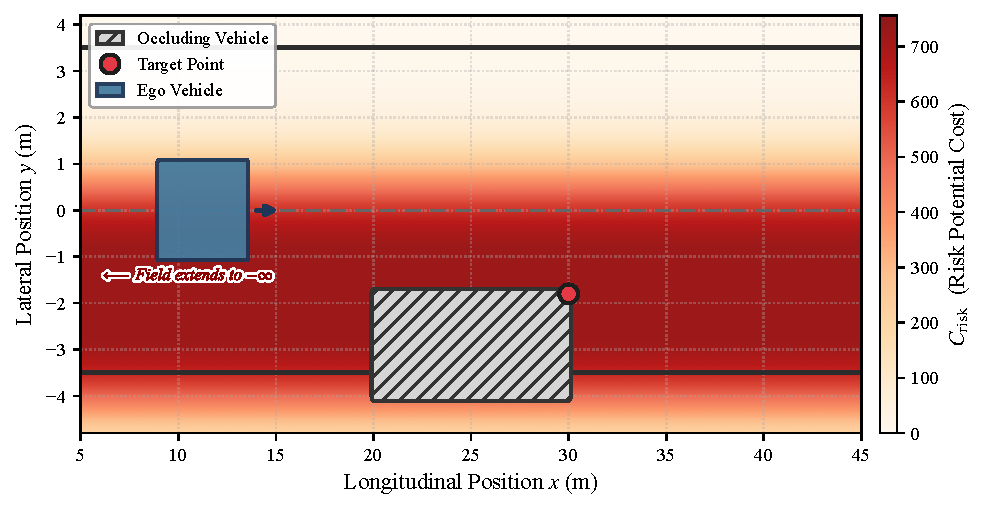
\includegraphics[width=\columnwidth]{figures/risk_field_academic.pdf}
\caption{PA-LOI 速度感知风险场的热力分布示意图。Target Point 位于右侧停放遮挡物的邻车道侧前角。惩罚区域沿纵向无限延伸（图中因截取而有限显示），确保 iLQR 在整个预测窗口内均接收到超速惩罚的梯度信号。}
\label{fig:risk_field}
\end{figure}

\subsection{底层 AEB 安全防线}
PA-LOI 作为前置调节层为 AEB 提供速度缓冲。当估算的碰撞时间 $TTC$ (Time-To-Collision) $\leq \SI{1.4}{\second}$ 时，底层 AEB 强制介入实施全力制动。本文将 AEB 可用的最大制动减速度设定为 $a_{\text{max}} = \SI{-4.0}{\meter\per\second\squared}$，该值显著低于干燥路面下的典型制动能力（$\SI{8}{\meter\per\second\squared}\sim\SI{10}{\meter\per\second\squared}$），旨在模拟雨雪等低附着系数极端路面条件，以此检验系统在最不利物理约束下的防护能力。前述 $v_{\text{safe}}$ 的推导同样基于该保守设定，确保安全车速包络与场景假定的可用制动力始终匹配。

% ============================================================
% IV. Experimental Setup
% ============================================================
\section{实验评估与部署环境 (Experimental Setup)}

所有仿真实验及计算耗时测量均在配备 Apple M3 芯片（8核，4性能核 + 4效能核）、16\,GB 统一内存的 MacBook Air 上完成，不依赖任何外部 GPU 加速。

\subsection{仿真环境与典型测试场景}
实验基于 Argoverse 2~\cite{argoverse2} 仿真环境，以 \SI{10}{\hertz} 的闭环频率运行。我们构建了两类典型的遮挡横穿测试场景（如图~\ref{fig:scenarios}）：
\begin{enumerate}
    \item \textbf{直道连续停车场景}（图~\ref{fig:scenarios}a）：道路右侧存在连续停放的大型车辆，形成较长的遮挡区域。自车以约 \SI{8.0}{\meter\per\second} 的巡航速度行驶。
    \item \textbf{路口遮挡场景}（图~\ref{fig:scenarios}b）：典型城市十字路口，因排队等候车辆在路口形成多处视线遮挡区域，自车以约 \SI{4.5}{\meter\per\second} 的较低速度通过。
\end{enumerate}

\begin{figure}[ht]
    \centering
    \subfloat[Straight road]{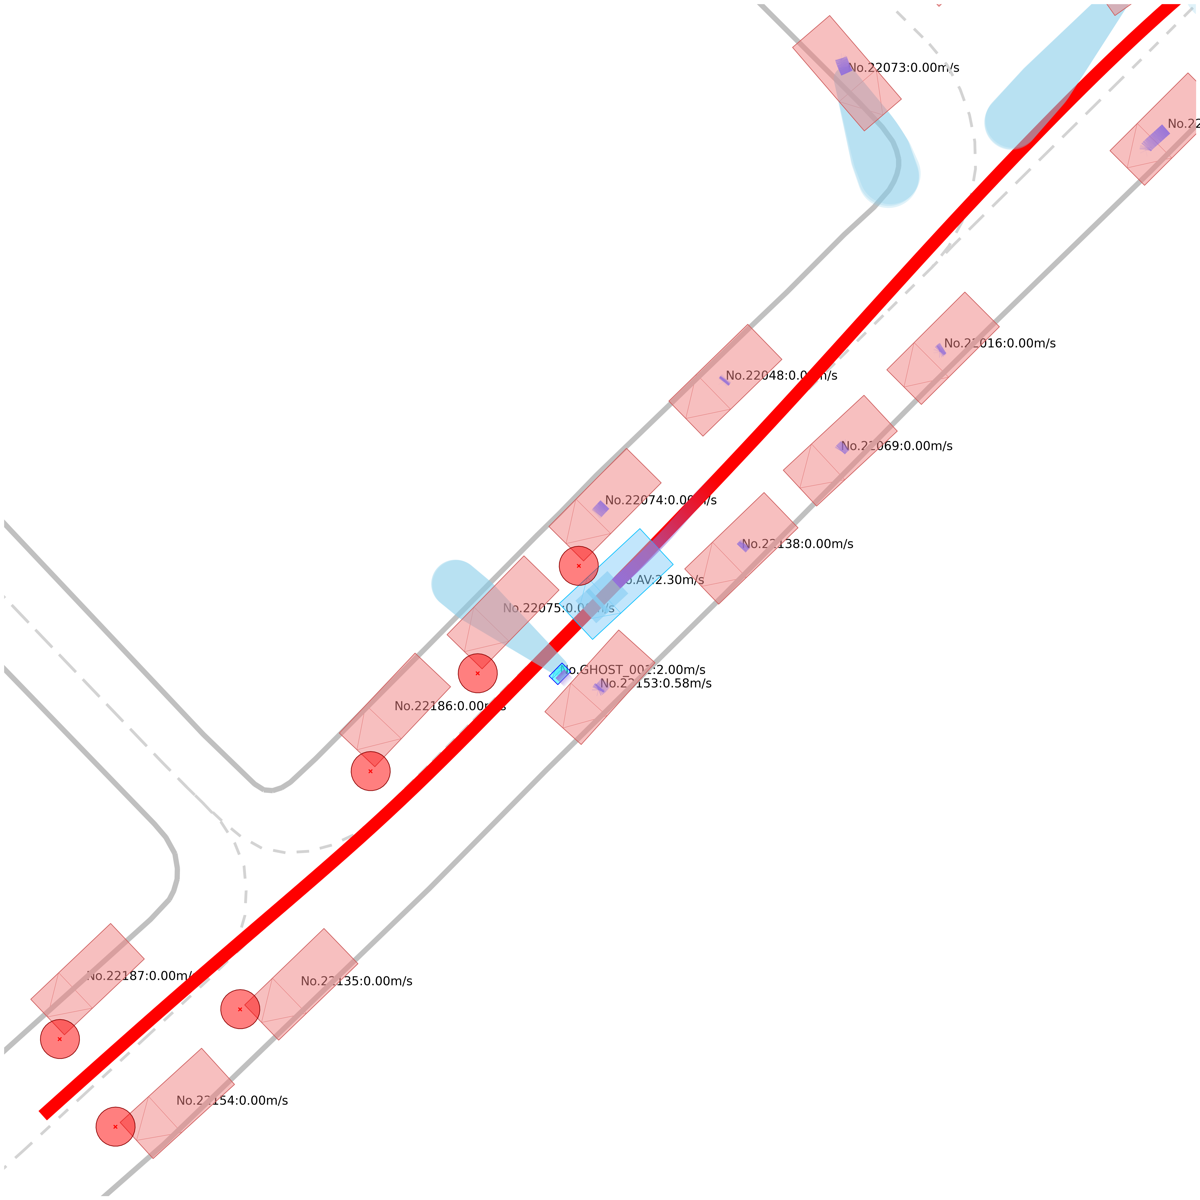
\includegraphics[width=0.48\columnwidth]{figures/straight_road.png}}
    \hfill
    \subfloat[Complex intersection]{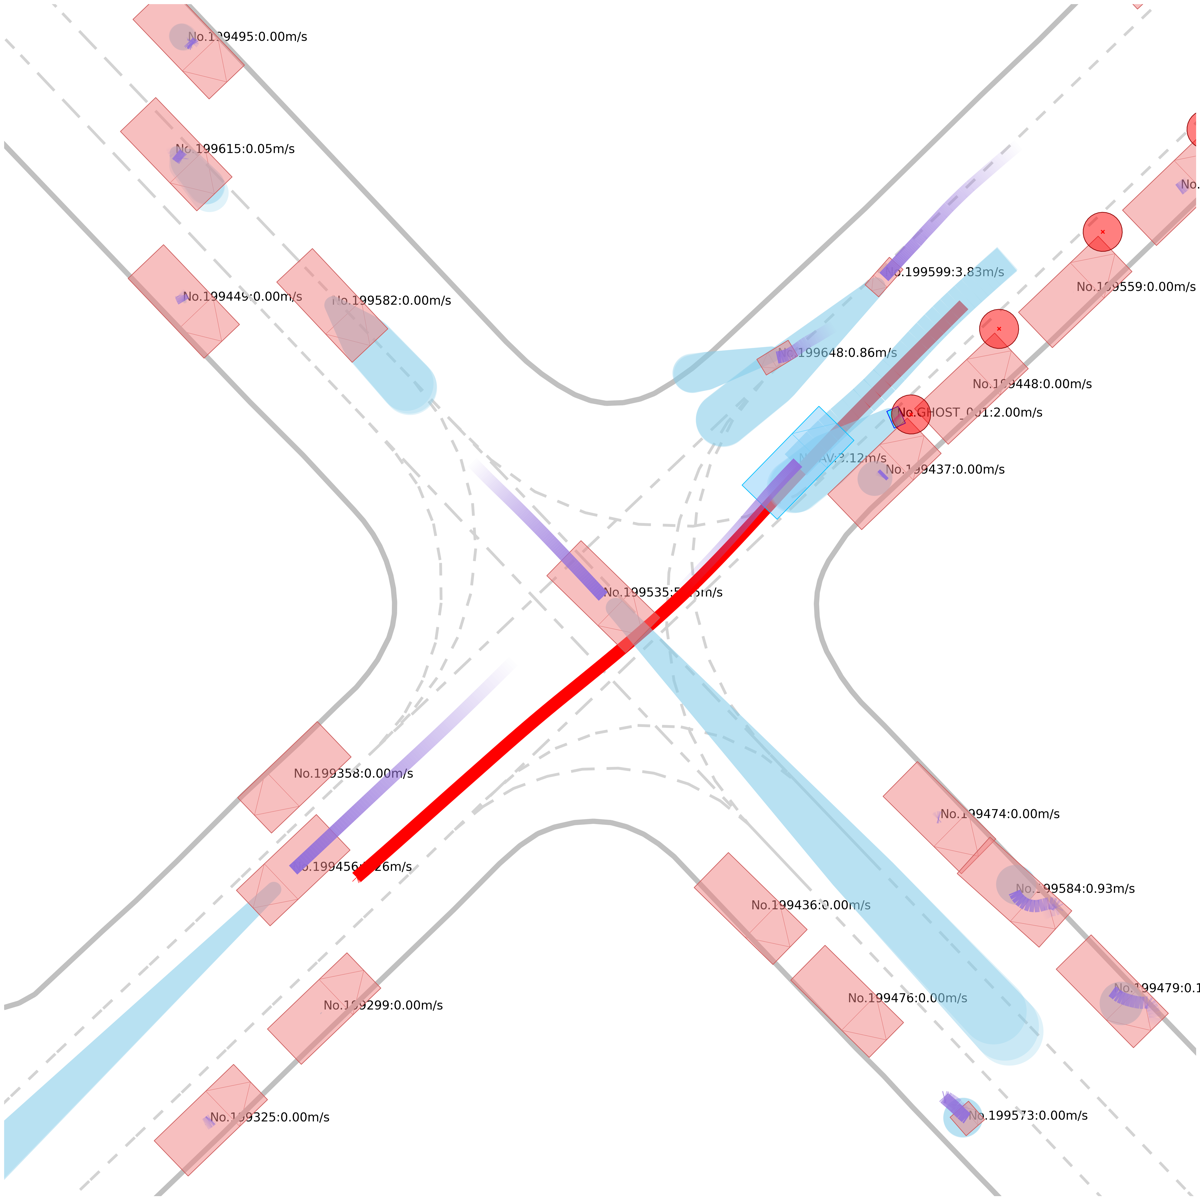
\includegraphics[width=0.48\columnwidth]{figures/intersection.png}}
    \caption{两类代表性的遮挡横穿挑战场地。(a) 右侧带较深连续静止车辆停放的城市道路段环境。(b) 由于相邻队列拥堵带来的典型十字路口内部车流视野截断。}
    \label{fig:scenarios}
\end{figure}

本系列测试的触发条件参考了 CPNA 标准测试规范，设计为当自车越过触发预先设定的关键物理间距 ($d_{\text{trigger}}$) 后的下一个执行帧内，目标隐蔽行人即刻以 \SI{2.0}{\meter\per\second} 的横向速度斜切进自车行驶车道并停留于车道内。这一最恶劣情况简化假设——行人停在车道中央而非继续横穿——最大化了与自车轨迹的时空重叠，确保除非自车已提前完成预防性减速，否则几何碰撞在物理上不可避免。

\subsection{评估系统控制组}
为全面展示该系统在动态场景中的优势，实验包含如下评估基线配置：
\begin{enumerate}
    \item \textbf{原生架构 (Vanilla MIND)}：未经修改的原版 MIND 框架~\cite{mind2025}，不包含任何遮挡感知或主动减速模块，作为评测基线。
    \item \textbf{纯 AEB 模式 (AEB Only)}：在原生规划器输出端附加反应式 AEB，当 $TTC \leq \SI{1.4}{\second}$ 时以 \SI{-4.0}{\meter\per\second\squared} 的固定减速度实施紧急制动。
    \item \textbf{主被动联合 (PA-LOI + AEB)}：在规划层集成本文提出的 PA-LOI 模块，同时保留底层 AEB 作为最终安全防线。
    \item \textbf{保守基线 (Conservative WCA)}：基于责任敏感安全模型 (RSS)~\cite{shalev2017rss} 的最坏情况假设构建的极端保守基线。该配置假定所有遮挡区域均存在即时横穿威胁，在任何可能的交汇点前均强制将车速降至安全停车速度以下，代表了安全性上界但牺牲了通行效率。
\end{enumerate}

% ============================================================
% V. Results
% ============================================================
\section{实验评估结果与研讨 (Experimental Results)}

\subsection{各测试场景下的定量碰撞衰减评估}
两组测试场景的详细定量评估结果分别列于表~\ref{tab:results_intersection} 和表~\ref{tab:results_straight}。

\begin{table}[htbp]
\caption{多变路口场景避让效能评估结果}
\label{tab:results_intersection}
\centering
\renewcommand{\arraystretch}{1.15}
\resizebox{\columnwidth}{!}{
\begin{tabular}{cc|cc|cc|cc|cc}
\toprule
\multirow{2}{*}{\shortstack{$d_{\text{trigger}}$\\(m)}} & 
\multirow{2}{*}{\shortstack{$d_{\text{bumper}}$\\(m)}} & 
\multicolumn{2}{c|}{Vanilla} & 
\multicolumn{2}{c|}{AEB Only} & 
\multicolumn{2}{c|}{PA-LOI+AEB} &
\multicolumn{2}{c}{Cons.\ WCA} \\
& & Col. & $v_{\text{imp}}$ & Col. & $v_{\text{imp}}$ & Col. & $v_{\text{imp}}$ & Col. & $v_{\text{imp}}$ \\
\midrule
3.0 & 0.75 & \xmark & 4.59 & \xmark & 3.99 & \xmark & 2.94 & \cmark & -- \\
3.5 & 1.25 & \xmark & 4.53 & \xmark & 3.96 & \xmark & 2.79 & \cmark & -- \\
4.0 & 1.75 & \xmark & 4.57 & \xmark & 3.46 & \xmark & 2.33 & \cmark & -- \\
4.3 & 2.05 & \xmark & 4.55 & \xmark & 2.88 & \xmark & 1.62 & \cmark & -- \\
4.5 & 2.25 & \xmark & 4.49 & \xmark & 2.88 & \cmark & -- & \cmark & -- \\
5.0 & 2.75 & \xmark & 4.60 & \xmark & 2.15 & \cmark & -- & \cmark & -- \\
5.5 & 3.25 & \xmark & 4.66 & \cmark & -- & \cmark & -- & \cmark & -- \\
\bottomrule
\end{tabular}
}
\vspace{1mm}
\footnotesize{注：Col. 标示碰撞是否发生 (\xmark: 发生碰撞, \cmark: 成功安全规避); $v_{\text{imp}}$ 反映碰撞实际留存末端速度 (m/s).}
\end{table}

\begin{table}[htbp]
\caption{直道长距离视线阻隔测试通过率与衰减对比}
\label{tab:results_straight}
\centering
\renewcommand{\arraystretch}{1.15}
\resizebox{\columnwidth}{!}{
\begin{tabular}{cc|cc|cc|cc|cc}
\toprule
\multirow{2}{*}{\shortstack{$d_{\text{trigger}}$\\(m)}} & 
\multirow{2}{*}{\shortstack{$d_{\text{bumper}}$\\(m)}} & 
\multicolumn{2}{c|}{Vanilla} & 
\multicolumn{2}{c|}{AEB Only} & 
\multicolumn{2}{c|}{PA-LOI+AEB} &
\multicolumn{2}{c}{Cons.\ WCA} \\
& & Col. & $v_{\text{imp}}$ & Col. & $v_{\text{imp}}$ & Col. & $v_{\text{imp}}$ & Col. & $v_{\text{imp}}$ \\
\midrule
3.0 & 0.75 & \xmark & 7.75 & \xmark & 7.67 & \xmark & 2.26 & \cmark & -- \\
3.5 & 1.25 & \xmark & 7.75 & \xmark & 7.27 & \xmark & 1.23 & \cmark & -- \\
4.0 & 1.75 & \xmark & 7.75 & \xmark & 7.27 & \cmark & -- & \cmark & -- \\
4.5 & 2.25 & \xmark & 7.75 & \xmark & 6.87 & \cmark & -- & \cmark & -- \\
5.0 & 2.75 & \xmark & 7.75 & \xmark & 6.39 & \cmark & -- & \cmark & -- \\
\bottomrule
\end{tabular}
}
\vspace{1mm}
\footnotesize{注：Conservative WCA 在所有工况下均因极端保守的速度策略而未发生碰撞。}
\end{table}

\subsection{对于制动边界的安全扩展验证}
实验数据表明，单独部署 AEB（AEB Only）在高速直道场景中存在明显的防护局限。在约 \SI{7.75}{\meter\per\second} 的初始车速下，由运动学制动公式 $d_{\text{brake}} = v^2 / (2a_{\text{max}})$ 计算可得最小制动距离约为 $\SI{7.51}{\meter}$，这远超本次实验预设的 \SIrange{3.0}{5.0}{\meter} 触发距离范围，因此单独 AEB 在该场景下的所有测试中均无法避免碰撞。

引入 PA-LOI 后，系统展现出显著的安全余量扩展：在路口场景中，PA-LOI+AEB 将实现零碰撞所需的最小前保险杠净距从单独 AEB 的 \SI{3.25}{\meter} 缩减至 \SI{2.25}{\meter}，安全缓冲距离改善约 \textbf{31\%}。在高速直道场景中，PA-LOI+AEB 在触发距离 \SI{4.0}{\meter}（前保险杠净距 \SI{1.75}{\meter}）下仍可实现零碰撞，而单独 AEB 在所有测试距离下均未能避免碰撞。即使在最极端的 \SI{3.0}{\meter} 近距触发工况下碰撞不可避免，PA-LOI 仍通过前置降速将碰撞末速从 \SI{7.75}{\meter\per\second} 降至 \SI{2.26}{\meter\per\second}，碰撞动能降低约 \textbf{91\%}。

值得注意的是，Conservative WCA 虽然在所有工况下均可实现零碰撞，但其代价是对所有遮挡区域采取无差别强制减速，这在正常交通流中将严重降低通行效率（即使在没有实际威胁的情况下，它也频繁导致车辆近乎完全刹停）。相比之下，PA-LOI 在安全性与通行效率之间实现了更为有利的折中：与未修改的基线相比，以仅新增 \SI{0.55}{\milli\second} 的计算开销为代价，它提供了接近保守基线的安全收益。主动减速自然受到 TTA 门控机制的限制，确保降速仅在物理上必要的窗口内接合，而不会导致长时间的低速爬行。



\subsection{计算开销与误报抑制}
验证系统在无真实威胁时不会引发过度减速（即误报抑制能力）对于实际部署至关重要。我们在无行人刷出的十字路口场景中进行了一次专门的 500 帧（\SI{50}{\second}）无威胁测试。在整个测试过程中，自车未表现出任何幽灵制动（phantom braking）事件或剧烈的轨迹扰动；它仅在接近遮挡交汇线时平缓降速，并在通过后恢复正常巡航。由于 PA-LOI 的 TTA 门控机制将干预严格限制在遮挡区附近的狭窄时间窗口内，同时 Hinge-Loss 的零梯度属性确保了在车速已经低于安全阈值时不会产生额外惩罚，该系统带来的全轨迹平均速度损失与无保护的 Vanilla MIND 基线相比不超过 1.5\%。

在计算开销方面，PA-LOI 模块单帧新增耗时仅约 \SI{0.55}{\milli\second}（亚毫秒级），满足典型 $10\sim\SI{20}{\hertz} $ 闭环自动驾驶系统的实时性需求。

\subsection{系统组件消融研究}
为验证组件的必要性，我们在 \SI{4.5}{\meter} 触发距离下进行了消融实验，结果如表~\ref{tab:ablation} 所示。
(1) \textbf{去除 TTA 筛选 (w/o TTA Screening)}：移除时间约束会导致系统退化为静态空间场，引发极端的"幽灵停滞 (Freeze-Robot)"异常。自车在远达 \SI{16.6}{\meter} 处过早启动减速，以约 \SI{2.0}{\meter\per\second} 的龟速伴随更剧烈的转向修正持续爬行，在 \SI{6.0}{\second} 的正常通行窗口内甚至未能抵达触发区。这种过度保守严重破坏了通行效率。
(2) \textbf{去除合页损失 (w/o Hinge-Loss)}：用常规空间常量惩罚替换速度解耦的 Hinge-Loss 会剥夺优化器的主动"降速梯度激励"。由于空间惩罚不随车速衰减，自车陷入拒绝主动减速的困境，保持高速直到距盲区仅 \SI{5.1}{\meter} 时规划器才开始施加迟缓的制动。巨大的运动学亏空导致其最终以 \SI{2.50}{\meter\per\second} 发生碰撞。
这些结果证明了，TTA 对于防止幽灵刹车与维持时效性不可或缺，而 Hinge-Loss 提供了促使车辆平稳收敛至安全初速的关键优化激励。

\begin{table}[htbp]
\caption{在 \SI{4.5}{\meter} 触发距离下的消融实验结果}
\label{tab:ablation}
\centering
\renewcommand{\arraystretch}{1.15}
\resizebox{\columnwidth}{!}{
\begin{tabular}{lccc}
\toprule
\textbf{评估指标} & \textbf{Full PA-LOI} & \textbf{w/o TTA} & \textbf{w/o Hinge-Loss} \\
\midrule
碰撞结果        & \textbf{安全通过} & 安全 (超时未达) & \textbf{发生碰撞} (\SI{2.50}{\meter\per\second}) \\
首次减速距离    & \textbf{12.2 m} & 16.6 m (过早) & 5.1 m (过晚) \\
路口最低车速    & \textbf{0.14 m/s} & 2.03 m/s & 0.82 m/s \\
转向抖动 (Std.) & \textbf{1.00} & 1.07 (+7\%) & 1.09 (+9\%) \\
\bottomrule
\end{tabular}
}
\end{table}

% ============================================================
% VI. 讨论与局限性 (Discussion)
% ============================================================
\section{讨论与局限性 (Discussion \& Limitations)}

实验结果表明，在反应式 AEB 制动基础上叠加前馈式的主动速度管理，可在保持正常通行效率的同时显著扩展系统的安全制动包络。这种"前馈降能 + 反应式制动"的双层协同架构，为解决 CPNA 等遮挡横穿类极端场景提供了一条有效的技术路径。

本方法目前存在以下局限：(1) 风险点的锚定依赖于对静态遮挡物的准确检测与定位，尚未考虑动态遮挡物（如行驶中的大型车辆）的处理；融合目标轨迹预测以拓展 PA-LOI 对动态遮挡的处理能力是一个极具潜力的未来方向。(2) 尽管实验表明系统在 $1.0\sim\SI{3.0}{\meter\per\second}$ 的行人速度范围内表现稳定，但尚未针对骑行等极端高速横穿模式（$>\SI{5.0}{\meter\per\second}$）进行验证，此类场景可能超出当前安全缓冲的覆盖范围；(3) 实验仅在仿真环境中进行了验证，尚需在实车平台上进一步评估。未来工作可结合 V2X 通信或非视距感知技术扩展遮挡信息来源，并引入行人意图预测模型以提升 $v_{\text{safe}}$ 估算的精度。

此外，关于实验配置方面，本研究将 AEB 可用的制动减速度限制在 \SI{-4.0}{\meter\per\second\squared}，旨在模拟具有挑战性的低附着力路面条件（如雨雪天气）。尽管现代 AEB 系统在干燥的高附着力路面上能够爆发出高达 \SI{-8.0}{\meter\per\second\squared} 的制动力（这通常足以独立避免碰撞），但 PA-LOI 的主动车速管理在这些理想环境下依然具有极高的价值。通过平滑地预先衰减行进车速，PA-LOI 能够将原本极其剧烈、严重影响乘员体验的紧急制动事件，转化为更为温和柔顺的减速曲线，从而在日常驾驶场景中显著提升乘坐舒适感与乘员的系统信任度。

% ============================================================
% VII. 结论 (Conclusion)
% ============================================================
\section{结论 (Conclusion)}

本文提出了 PA-LOI，一种面向视线受阻横穿场景的轻量化主动速度管理框架。该方法通过基于 TTA 的物理可达性评估动态界定安全车速，并以速度解耦的合页损失代价函数替代传统空间排斥势场，在避免轨迹振荡与优化死锁的同时实现了对盲区交汇前车速的平滑抑制。实验表明，PA-LOI 协同 AEB 在复杂路口场景中可将安全缓冲距离改善约 \textbf{31\%}，并在高速直道的最恶劣工况下将碰撞动能降低约 \textbf{91\%}，同时保持单帧仅 \SI{0.55}{\milli\second} 的极低计算开销。该框架可作为独立模块嵌入现有规划架构，为城市复杂环境下的遮挡行人防护提供了一种高效且实用的前置风控方案。

% ============================================================
% References
% ============================================================
\bibliographystyle{IEEEtran}
\bibliography{references}

\end{document}
